\documentclass{article}
\usepackage[utf8]{inputenc}
\usepackage[siunitx]{circuitikz}
\usepackage{amsmath}
\usepackage{wrapfig}
\usepackage{graphicx}
\usepackage{pgfplots}
\usepackage{float}
\usepackage[a4paper, total={6in, 8in}]{geometry}

\pgfplotsset{compat=1.18}

\title{Hardverski interfejsi - domaći zadatak}
\author{Nenad Radović, RA18/2020}
\date{01. april, 2023. godina}

\begin{document}

    \maketitle
    \renewcommand{\figurename}{Slika}
    \section{Problem i prijedlog rješenja}

    \begin{figure}[ht]

        \centering

        \begin{circuitikz}[american]
            
            \draw
            (0, 3) node[label=west:$V_1$] {}
            (0, 3) to[full diode, o-, v>=$V_{D_1}$, label=$D_1$] (3, 3)
            (6, 3) node[label=north:$A$] {}
            (3, 3) to[R, -*, v>=$V_{R_1}$, i=$I_1$, label=$R_1$] (6, 3)
            (6, 0) node[label=south:$V_2$] {}
            (6, 0) to[full diode, o-, v>=$V_{D_2}$, i=$I_2$, label=$D_2$] (6, 3)
            (9, 3) node[label=south:$B$] {}
            (6, 3) to[R, -*, v>=$V_{R_2}$, i=$I_3$, label=$R_2$] (9, 3)
            (9, 6) node[label=north:$V_3$] {}
            (9, 3) to[full diode, -o, v>=$V_{D_3}$, i=$I_4$, label=$D_3$] (9, 6)
            (12, 3) node[label=east:$V_4$] {}
            (9, 3) to[R, -o, v>=$V_{R_3}$, i=$I_5$, label=$R_3$] (12, 3);

        \end{circuitikz}

        \caption{Slika problema}

    \end{figure}

    Na slici 1, pored datih \textbf{napona $V_1$, $V_2$, $V_3$ i $V_4$}, obilježimo i padove na svim
    ostalim elementima (otpornicima i diodama) u kolu, kao i smjerove struja.

    Kako u kolu imamo $3$ diode, imamo $3^2 = 9$ mogućih pretpostavki o tome da li diode provode ili ne.
   
    Kao prvu pretpostavku, razmatraćemo da sve diode provode. Vidjećemo da ta pretpostavka nije tačna, ali će nas navesti
    na drugu koja se ispostavlja validnom.

    \newpage

    \subsection{Pretpostavka 1 - Sve diode provode}

        Ako sve diode provode, padovi napona na njima su $V_{D_1} = V_{D_2} = V_{D_3} = V_{D} = 0.5\si{\volt}$ (po postavci zadatka).
        
        Način na koji ćemo provjeriti da li je naša pretpostavka validna jeste što ćemo gledati smjerove struja.
        Ako se dobijeni smjerovi struja ne poklapaju sa onima označenim na slici, naša pretpostavka nije tačna.

        Gledajući sa slike, možemo zapisati prvi (strujni) Kirhofov zakon za tačke $A$ i $B$:

            \begin{align}
                I_1 + I_2 - I_3 = 0 \label{eq1} \\
                I_3 - I_4 - I_5 = 0 \label{eq2}
            \end{align}

        Napišimo drugi (naponski) Kirhofov zakon za sledeći dio kola:

        \begin{equation}
            \begin{split}
                V_1 - V_{D_1} - R_1I_1 + V_{D_2} - V_2 = 0 \\
                I_1 = \frac{V_1 - V_{D_1} + V_{D_2} - V_2}{R_1} \\
                I_1 = 1.66\si{\mA}
            \end{split}
            \label{eq3}
        \end{equation}
        
        \begin{figure}[ht]

            \centering

            \begin{circuitikz}[american]

                \draw 
                (0, 3) node[label=west:$V_1$] {}
                (0, 3) to[full diode, o-, v>=$V_{D_1}$, label=$D_1$] (3, 3)
                (6, 3) node[label=north:$A$] {}
                (3, 3) to[R, -*, v>=$V_{R_1}$, i=$I_1$, label=$R_1$] (6, 3)
                (6, 0) node[label=south:$V_2$] {}
                (6, 0) to[full diode, o-, v>=$V_{D_2}$, i=$I_2$, label=$D_2$] (6, 3);
        
            \end{circuitikz}

            \caption{Kontura $C_1$, podaci: $V_1 = 10 \si{\volt}$, $V_2=5 \si{\volt}$, $V_{D_1} = V_{D_2} = 0.5 \si{\volt}$, $R_1 = 3 \si{\kohm}$}

        \end{figure}

        Za struju $I_1$, koja prolazi kroz diodu $D_1$ dobijamo pozitivnu vrijednost, što znači da dioda provodi i da je 
        direktno polarisana, kao i po pretpostavci.

        Uradimo slično i za konturu $C_2$:

        \begin{figure}[ht]

            \centering

            \begin{circuitikz}[american]

                \draw 
                (9, 3) node[label=south:$B$] {}
                (9, 6) node[label=north:$V_3$] {}
                (9, 3) to[full diode, -o, v>=$V_{D_3}$, i=$I_4$, label=$D_3$] (9, 6)
                (12, 3) node[label=east:$V_4$] {}
                (9, 3) to[R, *-o, v>=$V_{R_3}$, i=$I_5$, label=$R_3$] (12, 3);
        
            \end{circuitikz}

            \caption{Kontura $C_2$, podaci: $V_3 = 0 \si{\volt}$, $V_4 = -5 \si{\volt}$, $V_{D_3} = 0.5 \si{\volt}$, $R_3 = 2.5 \si{\kohm}$}

        \end{figure}

        \begin{equation}
            \begin{split}
                -R_3I_5 - V_4 + V_3 + V_{D_3} = 0 \\
                I_5 = \frac{- V_4 + V_3 + V_{D_3}}{R_3} \\
                I_5 = 2.2 \si{\mA}
            \end{split}
            \label{eq4}
        \end{equation}

        \newpage

        Naredni korak je da izračunamo struju $I_3$, koja nam otvara put da iskoristimo jednačine (\ref{eq1}).
        Kako bismo nju izračunali, potrebno je naći napone u tačkama $A$ i $B$.

        Sa slike 1 uočavamo da je napon u tački $A$ napon katode diode $D_2$, kao i da 
        je napon u tački $B$ napon anode diode $D_3$. Poznavajući iznose padova napona na diodama, dobijamo sledeće:


        \begin{equation}
            \begin{split}
                V_2 - V_A = V_{D_2} \\
                V_A = V_2 - V_{D_2} \\
                V_A = 4.5 \si{\volt}
            \end{split}
            \label{eq5}
        \end{equation}

        \begin{equation}
            \begin{split}
                V_B - V_3 = V_{D_3} \\
                V_B = V_3 + V_{D_3} \\
                V_B = 0.5 \si{\volt}
            \end{split}
            \label{eq6}
        \end{equation}

        Struja na otporniku $R_2$ je naša tražena struja $I_3$, pa slijedi:

        \begin{equation}
            \begin{split}
                V_A - V_B = R_2I_3 \\
                I_3 = \frac{V_A - V_B}{R_3} \\
                I_3 = 0.57 \si{\mA}
            \end{split}
        \end{equation}

        Iz jednačina (\ref{eq1}) i (\ref{eq2}) dobijamo iznose struja $I_2$ i $I_4$:

        \begin{align} 
            I_2 = -1.09 \si{\mA} \label{eq7} \\ 
            I_4 = -1.63 \si{\mA} \label{eq8}
        \end{align}

        Dobili smo da su struje negativnog predznaka, što se kosi sa postavljenim smjerom struja kroz diode.

        Naša pretpostavka nije validna, ali nas navodi na drugu pretpostavku - da diode $D_2$ i $D_3$ ne provode, dok $D_1$ provodi.

        \newpage

    \subsection{Pretpostavka 2 - Dioda $D_1$ provodi, dok diode $D_2$ i $D_3$ ne provode}

        Kako pomenute diode ne provode, struje u granama u kojima se one nalaze jednake su nuli. 
        Kolo koje tada posmatramo izgleda kao:
        
        \begin{figure}[ht]

            \centering
    
            \begin{circuitikz}[american]
                
                \draw
                (0, 3) node[label=west:$V_1$] {}
                (0, 3) to[full diode, o-, v>=$V_{D_1}$, label=$D_1$] (3, 3)
                (6, 3) node[label=north:$A$] {}
                (3, 3) to[R, -*, v>=$V_{R_1}$, i=$I_1$, label=$R_1$] (6, 3)
                (6, 0) node[label=south:$V_2$] {}
                (6, 0) to[short, o-o] (6, 1)
                (6, 2) to[short, o-*] (6, 3)
                (9, 3) node[label=south:$B$] {}
                (6, 3) to[R, -*, v>=$V_{R_2}$, i=$I_1$, label=$R_2$] (9, 3)
                (9, 6) node[label=north:$V_3$] {}
                (9, 3) to[short, *-o] (9, 4)
                (9, 5) to[short, o-o] (9, 6)
                (12, 3) node[label=east:$V_4$] {}
                (9, 3) to[R, -o, v>=$V_{R_3}$, i=$I_1$, label=$R_3$] (12, 3);
    
            \end{circuitikz}
    
            \caption{Izgled kola po uslovima pretpostavke 1.2}
    
        \end{figure}

        Struktura sa slike 4 je dosta direktna - kroz nju teče jedna struja $I_1$ i jednačina koja je opisuje je sledeća:

        \begin{equation}
            V_1 - V_{D_1} - (R_1 + R_2 + R_3)I_1 - V_4 = 0
            \label{eq9}
        \end{equation}

        Iz jednačine (\ref{eq9}) izvućićemo vrijednost struje $I_1$:

        \begin{equation}
            \begin{split}
                I_1 = \frac{V_1 - V_{D_1} - V_4}{R_1 + R_2 + R_3} \\
                I_1 = 1.16 \si{\mA}
                \label{eq10}
            \end{split}
        \end{equation}
        
        Poznavanje ove struje nam je potrebno kako bismo izračunali napone u tačkama $A$ i $B$. 
        Naponi u pomenutim tačkama predstavljaju napone anoda i katoda na diodama, baš kao i u prošloj pretpostavci (1.1).
        Oni moraju biti ispod $0.5 \si{\volt}$, kako bi naša pretpostavka (1.2) bila tačna.

        Slijedi da:

        \begin{equation}
            \begin{split}
                V_1 - V_{D_1} - R_1I_1 - V_A = 0 \\
                V_A = V_1 - V_{D_1} - R_1I_1 \\
                V_A = 6.02 \si{\volt}
                \label{eq11}
            \end{split}
        \end{equation}

        \begin{equation}
            \begin{split}
                V_1 - V_{D_1} - R_1I_1 - R_2I_1 - V_B = 0 \\
                V_B = V_1 - V_{D_1} - R_1I_1 - R_2I_1 \\
                V_B = -2.1 \si{\volt}
                \label{eq12}
            \end{split}
        \end{equation}

        U slučaju diode $D_2$, kao i u prethodnoj pretpostavci (1.1), njenu anodu predstavlja napon $V_2$, dok je katoda na naponu $V_A$, pa slijedi:
        
        \begin{equation}
            \begin{split}
                V_{D_2} = V_2 - V_A \\
                V_{D_2} = -1.02 \si{\volt}
            \end{split}
            \label{eq13}
        \end{equation}

        Zaista, napon na njoj je manji od $0.5 \si{\volt}$, što vodi do zaključka da dioda ne provodi.
        Sličan zaključak dobijamo i za diodu $D_3$:

        \begin{equation}
            \begin{split}
                V_{D_3} = V_B - V_3 \\
                V_{D_3} = -2.1 \si{\volt}
            \end{split}
            \label{eq14}
        \end{equation}

        Pretpostavka je potvrdjena. U daljem dijelu je ostalo da skiciramo radne tačke za diode, koje izgledaju:

        \begin{figure}[ht]
            \centering
                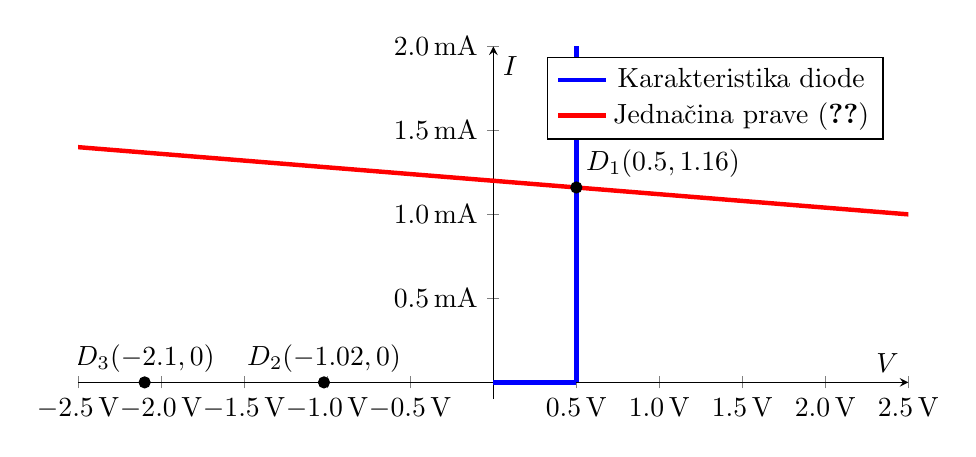
\begin{tikzpicture}
                    \begin{axis}[xmin = -2.5, xmax = 2.5, 
                                 ymin = -0.1, ymax = 2,
                                 width=\textwidth,
                                 height=0.5\textwidth,
                                 xlabel=$V$, ylabel=$I$,
                                 xticklabel={\SI[round-mode=places, round-precision=1]{\tick}{V}},
                                 yticklabel={\SI[round-mode=places, round-precision=1]{\tick}{mA}},
                                 samples=50, axis lines=middle,
                                 legend pos=north east]
        
                        \addplot[domain=0:0.5, blue, ultra thick] (x, 0);
                        \addplot[domain=0:4, blue, ultra thick] (0.5, x);
                        \addplot[red, ultra thick]{1.2 - x*0.08};
                        \filldraw[black] (0.5, 1.16) circle (2pt) node[anchor=south west]{$D_1(0.5, 1.16)$};
                        \filldraw[black] (-1.02, 0) circle (2pt) node[anchor=south]{$D_2(-1.02, 0)$};
                        \filldraw[black] (-2.1, 0) circle (2pt) node[anchor=south]{$D_3(-2.1, 0)$};
                        \legend{, Karakteristika diode, Jednačina prave (\ref{eq10})}
                    \end{axis}
                \end{tikzpicture}
                \caption{Radne tačke dioda}
        \end{figure}

\end{document}